\documentclass{article}
\usepackage{tikz}

\begin{document}

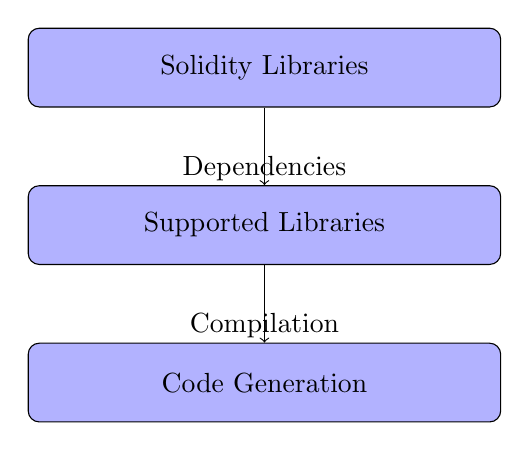
\begin{tikzpicture}[node distance=2cm]
    % Define styles for nodes
    \tikzstyle{stage} = [rectangle, draw, fill=blue!30, rounded corners, minimum width=6cm, minimum height=1cm]

    % Nodes for each stage
    \node (solidityLibraries) at (0,0) [stage] {Solidity Libraries};
    \node (supportedLibraries) at (0,-2) [stage] {Supported Libraries};
    \node (codeGeneration) at (0,-4) [stage] {Code Generation};

    % Connect nodes with arrows
    \draw[->] (solidityLibraries.south) -- node[midway, below] {Dependencies} (supportedLibraries.north);
    \draw[->] (supportedLibraries.south) -- node[midway, below] {Compilation} (codeGeneration.north);

\end{tikzpicture}

\end{document}